\documentclass{article}
\usepackage[utf8]{inputenc}
\usepackage[dvipsnames]{xcolor}
\usepackage{fullpage,amsmath,amssymb,graphicx,mathtools}
\usepackage[shortlabels]{enumitem}
\usepackage{amssymb,amsmath,amsfonts,bbm,epsf,graphicx,hyperref,pstricks,pgfplots,comment,color}
\usepackage[bottom]{footmisc}
\usepackage{todonotes}
\allowdisplaybreaks

\newif\ifsolutions
\newenvironment{labelledanswer}{{\bf Answer:} \sf }{}%                               
\newcommand{\answer}[2]
{{
\ifsolutions
\begin{labelledanswer}
\color{red} 
#2
\end{labelledanswer}
\else
#1
\fi
}}
\solutionstrue

\def\nexp{n}
\def\di{d}
\def\fm{p}

\title{CS229 Final Exam - Summer 2020}
\date{Aug 14 2020 7am PDT - Aug 15 2020 7am PDT}

\begin{document}

\maketitle

 This exam is open-notes and open-internet. However, any and all forms of online or offline discussion is prohibited (for instance, posting questions on StackExchange is not permitted). We expect the exam to be completable in roughly 3 hours, but are giving you a 24-hour submission window to accommodate various time zones and upload speeds onto Gradescope. Good luck!

\section*{[0 points] The Stanford University Honor Code}

At the top of your solution file, please write/type the following Honor Code statement and attest it (i.e. sign or print your name below it), thereby implying your consent to follow the code:

``\textit{I attest that I have not given or received aid in this examination, and that
I have done my share and taken an active part in seeing to it that others
as well as myself uphold the spirit and letter of the Honor Code.}''

\textbf{Submissions without the attested Honor Code statement will NOT be graded.}

``\textit{I attest that I have not given or received aid in this examination, and that
I have done my share and taken an active part in seeing to it that others
as well as myself uphold the spirit and letter of the Honor Code.}''\\

Anh Vu L. Nguyen

\clearpage

\section{[10 points] True or False}

Each question is worth 1 point. Provide a short justification (one or two lines) for each answer. There will be no negative points, but answers without justification will not receive credit.

\bigskip

\noindent For questions 1-3, consider a binary classification task where we have $n$ training examples, $x^{(i)} \in \mathbb{R}^d$, and hypothesis $h_\theta(x)$ is parameterized by $\theta$. 

\begin{enumerate}

\item \textbf{True or False}. Removing half the training data will increase variance.

\answer{}{True, this should mean that the model will have less to work with for prediction. The test prediction will likely be larger than before, indicating incrase variance.}

\item \textbf{True or False}. Removing half of the features of $x$ will increase bias.

\answer{}{True, this would increase bias since it forces the model to assume more with less information available.}

\item \textbf{True or False}. Removing half of the features of $x$ will increase variance.

\answer{}{False, removing features leads to increase in bias, which could lead to decrease in variance. }

\item \textbf{True or False}. Adding a constant to the arguments of Radial Basis Function (RBF) kernel will not change the value of the kernel.

\answer{}{True, since RBF kernels rely on calculating squared distance. This squared distance would be unchanged as $((x+c) - (x'+c))^2 = ((x - x')^2 $.}

\item \textbf{True or False}. The following probability density function parameterized by $\theta$ belongs to the exponential family.
\begin{align}
f(x;\theta) = \frac{\theta^x}{2\pi x^3}e^{-\theta}
\end{align}

\answer{}{False, $\theta^x$ is problematic here.}

\item \textbf{True or False}. When training a neural network, it is a good practice to initialize all weights to $0$.

\answer{}{False, we need random initialization. The reason is discussed in "Parameters Initialization" in Deep Learning Notes, but essentially to avoid the same output for first layer.}

\item \textbf{True or False}. There is a unique solution to $k$-means clustering regardless of how we initialize the $k$ centers. 

\answer{}{False, depending on how we initialize the $k$ centers, it'll impact the distance calculation to determine which group an examples belong to. This can in turn result in a different $k$-means solution as we run the algorithm each time through the same dataset.}

\end{enumerate}

\noindent For questions 8-10, suppose we train a SVM classifier to perform binary classification using hinge loss, i.e. 
\begin{align}
    L(y_i) = \max\{0, 1 - y_i (w^T x_i + b)\} 
\end{align}

\begin{enumerate}

\setcounter{enumi}{7}

\item \textbf{True or False}. Adding a regularization term to the loss function can change the decision boundary.

\answer{}{True, just like in class discussion on regularization and the non-separable case, this technique is used to make decision boundary less sensitive to outliers.}

\item \textbf{True or False}. Scaling each $x_i$ by constant $c$ can change the decision boundary.

\answer{}{False, since scaling all training data point by a constant c means that the distance from the points to decision boundary remains the same. SVM will again give us the same decision boundary.}

\item \textbf{True or False}. Removing all data points that are not support vectors (i.e., their distance from the decision boundary is greater than $1$) can change the decision boundary.

\answer{}{If done before introducing a new training, then True, because SVM would try to recreate the decision boundary using only the leftover points. However, if we mean that after we train, we only save the support vectors, and try to make prediction on a new point, then False, decision boundary remains the same.}

\end{enumerate}

\clearpage

\section{[10 points] Short Answers}

Each question is worth 2 points. Provide a short justification (one or two lines) for each answer.

\begin{enumerate}

\item \textbf{Short Answer}. 
What 3 components can Mean Squared Error be decomposed into? Which component can be reduced by using a larger training set? Which component can be reduced by adding another hidden layer in a neural net? Which component can be reduced by decreasing the dimension of parameter $\theta$?

\answer{}{
MSE =  Irreducible Error+ Bias$^2$ + Variance\\

Which component can be reduced by using a larger training set? Variance. This leads to the model potentially reduce the gap between cross-validation error and training error through learning from more examples.  \\
Which component can be reduced by adding another hidden layer in a neural net?  Bias. The model is now bigger and more complicated, leading it to learn more pontentially from its current set of features. Training error might be lower, indicating lower bias.\\
Which component can be reduced by decreasing the dimension of parameter $\theta$? This action would means that the parameter would have less expressive power. Depending on the data, this might cause it to perform worse on training error. An example if we're reducing parameters to 1 dimension, but we're predicting data that's much better expressed in 3 dimensions. Therefore, this seems to increase bias which might result in increase in variance. \\
}

\item \textbf{Short Answer}. 
How many parameters are necessary to specify a \emph{Bernoulli Event Model} Naive Bayes classifier with $c$ classes and vocabulary size $v$? Express your answer in terms of $c$ and $v$.

\answer{}{We would need $v\times c$ parameters in total.}

\item \textbf{Short Answer}.
Suppose we train a neural network to classify 16 x 16 pixel images into 4 classes. We flatten each image into a vector, and feed the images into a 3-layer neural net with 10 neurons in the first hidden layer, 6 neurons in the second hidden layer, and apply softmax loss at the output layer. How many parameters does this model have? (Don't forget to include biases!)

\answer{}{
For the first layer, the number of params = $(10 \times (16 \times 16)) + 10 = (10 \times 256) + 10$.\\
For the second layer, the number of params = $(6 \times 10) + 6$.\\
For the third layer, the number of params = $(4 \times 6) + 4$.\\
The model has 2664 parameters in total.\\\
}

\item \textbf{Short Answer}.
Consider a Markov Decision Process (MDP) defined as $(S, A, \{P_{sa}\}, \gamma, R)$, where $S$ is a finite set of $m$ states, $A$ is a finite set of $n$ actions, $\{P_{sa}\}$ are the transition probabilities, $\gamma$ is the discount factor, and $R$ is the reward function.
How many distinct deterministic policies $\pi:S\to A$ can be defined for this MDP?

\answer{}{
We can have up to $n^m$ policies. We have $n$ possible actions and $m$ states, and we can cycle through all $m$ states in the MDP with each state having $n$ possible actions (therefore, $n^m$).
}

\item \textbf{Short Answer}. Suppose we want to minimize a loss function parameterized by $\theta \in \mathbb{R}^d$, where $x \in \mathbb{R}^d$, $y \in \{-1, 1\}$, $z = y \theta^T x$, and the current value of z is -1.5. Which of the following loss functions would gradient descent fail to decrease, regardless of step size?
    \begin{enumerate}
        \item zero-one loss: $\varphi(z) = 1\{z \le 0\}$
        \item exponential loss: $\varphi(z) = e^{-z}$
        \item hinge loss: $\varphi(z) = \max\{1-z, 0\}$
    \end{enumerate}
\answer{}{
I found a good graphical plot for all these loss functions (source: https://rohanvarma.me/Loss-Functions): \\
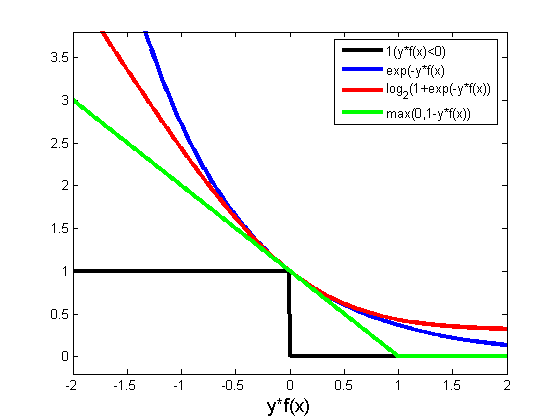
\includegraphics{loss_functions_q2_5.png} \\

(a) would not work here as the loss function is a straight line and does not have anything for gradient descent to work with. \\
(b) should work. \\
(c) should work since $z = -1.5$ currently. \\

}

\end{enumerate}

\clearpage

\section{[10 points] Theory \it{(Kernel Nearest Neighbor for Spam Classification)}}

In this problem, we will revisit the spam classification problem with the Kernel method. 

Recall that in homework 2 we implemented a Multinomial Event Model Naive Bayes classifier. Now we are going to combine the kernel method with the  K-nearest neighbor classification model. For simplicity, we use $k=1$ in the following scenario: for an incoming email, we calculate its kernel distance with each email in the training set, and assign the incoming email the label of the closest neighbor\footnote{If $k > 1$, we instead use the majority vote from the $k$ nearest neighbors as the predicted label.}. The performance of the algorithm highly depends on the kernel we choose, and we are going to compare options in this question.  

Let $S_i = [s_1, s_2, \cdots, s_{N_i}]$ be a string sequence (i.e. an email). Vocabulary $V$ is the set of all strings observed in any $S_i$. For a given sequence $S_i$, let $g_n(S_i)$ denote the set of all $n$-grams of $S_i$. For example,
    $$
        g_2([\text{I, saw, a, saw, that, saw, a, saw} ]) = \{\text{I saw},\,\text{saw a},\,\text{a saw},\,\text{saw that},\,\text{that saw}\}
    $$
    Notice here our 2-gram function only extracts one copy of `saw a' and `a saw'. Furthermore, we can define a string comparison function: 
\[
    \delta(s_j, s_k) =
\begin{cases}
  1,& \text{if } s_j = s_k\ \text{(i.e. the two n-gram strings are the same)}\\
    0,& \text{otherwise.}
\end{cases}
\]

\begin{itemize}
    \item [(a)] [4 points] 
    We define a kernel function as:
    $$
    K_{V,n}(S_1, S_2) = \sum_{x\in g_n(S_1)} \sum_{z\in g_n(S_2)} \delta(x, z)
    $$
    
    Express the kernel function using an appropriate feature mapping $\phi(S_i)$.
    That is, define the feature mapping $\phi(S_i) \in \mathbb{R}^d$ such that $K_{V,n}(S_1, S_2) = \phi(S_1)^\top\phi(S_2)$.
    What is the dimension of the feature mapping space $d$ in terms of $n$ and $V$?
    
    \emph{Hint}: The description of $\phi(S_i)$ should be brief.
    
    \answer{}{
 $$
    K_{V,n}(S_1, S_2) = \sum_{x\in g_n(S_1)} \sum_{z\in g_n(S_2)} \delta(x, z) = \sum_{x\in g_n(S_1)} \sum_{z\in g_n(S_2)} 1\{x=z\} = \sum_{x\in g_n(S_1)} \sum_{z\in g_n(S_2)} 1\{x=z\} \; 1\{z=x\}
 $$

The last equality is due the fact that if x=z then z=x as well. The operation here looks like we need to go through and count co-occurence between the two set of n-grams for $S_1, S_2$. 

%
%$$
%    K_{V,n}(S_1, S_2) = \sum_{x\in g_n(S_1)} \sum_{z\in g_n(S_2)} 1\{x=z\} \; 1\{z=x\} 
%$$
%$$
%= \sum_{i=1}^{l_1} \sum_{j=1}^{l_2} (1\{x=z\}) \; (1\{z=x\})
%$$
%Where $l_1 = len(g_n(S_1))$ and $l_2 = len(g_n(S_2))$.
%
%The feature map here is the p-spectrum kernels, where we can think each word as a character, and the entire string sequence as a string. This mapping makes sense since we don't particularly care about the length of each string within the string sequence. Instead, we care about matching subsequence of string of length n with another subsequence of string of length n. \\

The feature map is then $\phi(S_i) =  |{(n_1, n_2): s = n_1 \cup n_2}|$ \\

The feature map defined by this kernel associates each $S_i$ a vector of dimension $|V|^n$ containing the historgram of frequencies of all its substrings of length n (n-grams).
}
    
    \item[(b)] [3 points] In reality, the vocabulary size is usually large. For example {\it WikiText-103}, which contains all articles extracted from Wikipedia, has a vocabulary size of 217,646. However, the frequency of words has a long tail distribution and some of the words rarely appear. We can replace those rare words with a designated ``unknown token'' UNK to effectively reduce the vocabulary size. For example, if we restrict the vocabulary to $V'$ which only the has three tokens $\{ \text{I}, \text{saw}, \text{UNK}\}$, our previous example becomes: $S'_i = [\text{I, saw, UNK, saw, UNK, saw, UNK, saw}]$, and
    $$
        g_2(S'_i) = \{\text{I saw},\, \text{saw UNK}, \, \text{UNK saw}\}
    $$
    Let $V'$ be the reduced vocabulary, i.e. a subset of $\{V \cup \{\text{UNK})\}$.
    We define the kernel function for $V'$ as:
        $$
        K_{V', n}(S_1, S_2) = \sum_{x\in g_n(S'_1)} \sum_{z\in g_n(S'_2)} \delta(x, z)
    $$
    Is this still a valid kernel? If yes, express the kernel function using an appropriate feature mapping $\phi'(S_i)$ and state its relation with $\phi(S_i)$. If not, please give a counterexample.
    
    \answer{}{
This should still be a valid kernel mapping as nothing has fundamentally changed. All the rare words are mapped to the "unknown token" UNK for all string. In a way, the feature map here seems to combine 2 feature mapping, first map to UNK tokens, and then second part is the same as the part above.\\

The feature map is updated to be:  $\phi'(S_i) =  |{(n_1, n_2): s = n_1 \cup n_2}|$ \\
    }
    
    \clearpage  
    
    \item[(c)] [2 points] Which of the following is true for any $V'$? Give a short explanation. 
    \begin{enumerate}
        \item [(A).] $K_{V, n}(S_1, S_2) \geq K_{V', n}(S_1, S_2)$
        \item [(B).] $K_{V, n}(S_1, S_2) \leq K_{V', n}(S_1, S_2)$
        \item [(C).] $K_{V, n}(S_1, S_2) > K_{V', n}(S_1, S_2)$
        \item [(D).] $K_{V, n}(S_1, S_2) < K_{V', n}(S_1, S_2)$
        \item [(E).] None of the above
    \end{enumerate}
    
    \answer{}{
   The mapping to UNK should account for the common n-grams in the string. We can run through a couple of examples: \\
   Using the string $S_1$="I saw that that saw an apple", and create 2-grams. For the original case with $V$, we have:
    $$
        g_2([\text{I, saw, that, that, saw, an, apple} ]) = \{\text{I saw},\,\text{that that},\,\text{that saw},\,\text{saw an},\,\text{an apple}\}
    $$
   For the case with $V'=(\text{I, saw, UNK})$, we have:
   $$
        g_2([\text{I, saw, UNK, UNK, saw, UNK, UNK} ]) = \{\text{I saw},\,\text{UNK UNK},\,\text{UNK saw},\,\text{saw UNK}\}
    $$
   Test with a couple of string:\\
   
 $S_2$= (that saw) will give us $K_{V, 2}(S_1, S_2) = K_{V', 2}(S_1, S_2) = 1$\\
 $S_2$= (an apple) will give us $K_{V, 2}(S_1, S_2) = K_{V', 2}(S_1, S_2) = 1$\\
 $S_2$= (an apple, an orange) will give us $K_{V, 2}(S_1, S_2) = K_{V',2}(S_1, S_2) = 1$ since both (an apple, an orange) are mapped to a singular (UNK UNK) and will only be counted once. \\
 $S_2$= (an apple, that saw) will give us $K_{V,2n}(S_1, S_2) = K_{V', 2}(S_1, S_2) = 2$ since (an apple, that saw) are mapped to (UNK UNK, UNK saw), which are both counted.\\
However, \\
$S_2$= (an apple, that that) will give us $K_{V, 2}(S_1, S_2) =2 > K_{V', 2}(S_1, S_2) = 1$. For $V'$, (an apple, that that) is mapped to (UNK UNK), and is counted once as common string. For $V$, we count both "an apple" and "that that", giving us 2.\\
This can be thought of as a consequence of many to one mapping in $V'$. As to whether $K_{V, n}(S_1, S_2) < K_{V', n}(S_1, S_2)$ is possible, we look at the following example:\\
 $S_2$= (an orange) will give us $K_{V,2n}(S_1, S_2) = 0 < K_{V', 2}(S_1, S_2) = 1$ since (an orange) is mapped to (UNK UNK), which is counted for $V'$. $V$ maintains the original string, which then means it isn't counted for any common string here.

Therefore, answer is E here.


    }
    
    \item[(d)] [1 points] Now we will apply this kernel to our spam classification problem. We hope that the nearest neighbor found through $K_{V', n}$, which is computationally more efficient, is the same as the nearest neighbor from the kernel space defined by $K_{V, n}$. 
    
    For any sequence $S_i$ in the training set $\mathcal{S}_{\text{train}}$, denote its ground truth label as $y(S_i)$. The Kernel Nearest Neighbor prediction for $S_t$ in the test set is:
    \[
        f_{V, n}(S_t) = y\left(\text{arg} \max_{S_i \in \mathcal{S}_{\text{train}}}  K_{V, n}(S_i, S_t)\right)\\
    \]
    We hope to observe:
    \[
        f_{V', n}(S_t) = f_{V, n}(S_t)  \tag{$\ast$} \label{eq:star}
    \]
    for any reduced vocabulary $V'$.
    
    Unfortunately, this is not true. We observe a trade-off between computational cost and accuracy: the smaller the vocabulary, the less computation is needed, but the more likely we do not find the true nearest neighbor. However, as long as the new vocabulary set $V'$ is not too small, this is still a good approximate classification model. 
    
    Give a concrete counterexample to the equation ($*$). You can choose any vocabularies $V, V'$, and $n$ for your example.
    
    \answer{}{
    $$
    f_{V, n}(S_t) = y\left(\text{arg} \max_{S_i \in \mathcal{S}_{\text{train}}}  K_{V, n}(S_i, S_t)\right)
    $$
    $$
    f_{V', n}(S_t) = y\left(\text{arg} \max_{S_i \in \mathcal{S}_{\text{train}}}  K_{V', n}(S_i, S_t)\right)
    $$
    We want to give counte example to: 
    $$
    y\left(\text{arg} \max_{S_i \in \mathcal{S}_{\text{train}}}  K_{V, n}(S_i, S_t)\right) = y\left(\text{arg} \max_{S_i \in \mathcal{S}_{\text{train}}}  K_{V', n}(S_i, S_t)\right)
    $$
    Let's choose an example where $n = 1$, which means that we're just counting common word between two string for the kernel. Then let's take $V$ to be all the words in the English dictionary, while $V'=\{\text{UNK}\}$, effectively reduce the vocab to 1 words. It's easy to see here that for any string that's actually the same, meaning $y=1$, $V'$ will map that to just {UNK}, making the maximum count of common to be 1 (since we also don't extract multiple same copy from the prompt). 
Let's say we have 2 string to train with $S_1$=("A B C") and $S_2$=("A B B C D"). For $V$, we have 1-gram \{"A", "B", "C"\} and \{"A", "B", "C", "D"\}. For $V'$, we have 1-gram \{UNK\}.
$$
    f_{V, n}(S_1) = y\left(\text{arg} \max_{S_i \in \mathcal{S}_{\text{train}}}  K_{V, n}(S_i, S_1)\right) = y (3)
$$
$$
    f_{V', n}(S_1) = y\left(\text{arg} \max_{S_i \in \mathcal{S}_{\text{train}}}  K_{V', n}(S_i, S_1)\right) = y (1)
$$
$$
 \implies f_{V', n}(S_t) \neq f_{V, n}(S_t)
$$
    
    
    }
    
\end{itemize} 

\clearpage 

\section{[10 points] Theory + Coding  \it{(The Poetic Scientist)}}

In this question, you will train a neural network to help write poetry. The goal is to find words that sound similar to each other. Weak supervision is one approach to learn how phonetically close or far two words are: your model will learn from and predict whether two inputs are similar or different sounding. Consider a two-layer network parameterized as follows:

\begin{align}
    h^{[1]}(x) &= W^{[1]}x + b^{[1]}\\
    a^{[1]}(x) &= \sigma(h^{[1]}(x))\\
    h^{[2]}(x) &= W^{[2]}a^{[1]}(x) + b^{[2]}
\end{align}

Our training examples will now consist of \textit{pairs} of inputs along with a label for whether the inputs are similar or dissimilar: $(x^{(i)}_1, x^{(i)}_2, y^{(i)}) \in \mathbb{R}^{d} \times \mathbb{R}^d \times \{-1, 1\}$ where $-1$ indicates a dissimilar pair and $1$ a similar pair. Consider the following loss:

\begin{align}
    \ell(x_1, x_2, y; W, b) = \log\left(1 + \exp(-y{h^{[2]}(x_1)}^\top h^{[2]}(x_2))\right)
\end{align}

\noindent \text{Theory:} [6 points]

\begin{itemize}
    \item [(a)] [1.5 points] Consider the loss for a single example. Write the expressions for $\frac{\partial \ell}{\partial h^{[2]}(x_1)},  \frac{\partial \ell}{\partial h^{[2]}(x_2)}$. 
    
    \answer{}{

$$
\frac{\partial}{\partial h^{[2]}(x_1)} \ell(x_1, x_2, y; W, b)= \frac{1}{1 + \exp(-y{h^{[2]}(x_1)}^\top h^{[2]}(x_2))} \;  \left(  0 + \exp(-y{h^{[2]}(x_1)}^\top h^{[2]}(x_2)) (-y h^{[2]}(x_2))   \right)
$$
$$
= \frac{ (-y h^{[2]}(x_2)) e^{(-y{h^{[2]}(x_1)}^\top h^{[2]}(x_2))}}{1 + e^{(-y{h^{[2]}(x_1)}^\top h^{[2]}(x_2))}}
$$

$$
\frac{\partial}{\partial h^{[2]}(x_2)} \ell(x_1, x_2, y; W, b)= \frac{1}{1 + \exp(-y{h^{[2]}(x_1)}^\top h^{[2]}(x_2))} \;  \left(  0 + \exp(-y{h^{[2]}(x_1)}^\top h^{[2]}(x_2)) (-y {h^{[2]}(x_1))}^\top   \right)
$$
$$
= \frac{ (-y {h^{[2]}(x_1)}^\top) e^{(-y{h^{[2]}(x_1)}^\top h^{[2]}(x_2))}}{1 + e^{(-y{h^{[2]}(x_1)}^\top h^{[2]}(x_2))}} 
$$           
    }
    
    \item [(b)] [1.5 points] Express $\frac{\partial \ell}{\partial W^{[2]}}$, $\frac{\partial \ell}{\partial b^{[2]}}$ in terms of $\frac{\partial \ell}{\partial h^{[2]}(x_1)}$ and $\frac{\partial \ell}{\partial h^{[2]}(x_2)}$ and $a^{[1]}(x_1), a^{[1]}(x_2)$.
    
    \answer{}{
$$
    \ell(x_1, x_2, y; W, b) = \log\left(1 + \exp(-y{h^{[2]}(x_1)}^\top h^{[2]}(x_2))\right) 
$$
$$
= \log\left(1 + \exp(-y{(W^{[2]}a^{[1]}(x_1) + b^{[2]})}^\top  (W^{[2]}a^{[1]}(x_2) + b^{[2]}))\right)
$$
$$
= \log\left(1 + e^{{(-yW^{[2]}a^{[1]}(x_1)}^\top - {yb^{[2]}}^\top )  (W^{[2]}a^{[1]}(x_2) + b^{[2]})}\right)
$$
$$
= \log\left(1 + e^{{(-yW^{[2]}a^{[1]}(x_1)}^\top - {yb^{[2]}}^\top )  (W^{[2]}a^{[1]}(x_2) + b^{[2]})}\right)
$$   
    
    }
    
    \item [(c)] [1.5 points] Express $\frac{\partial \ell}{\partial h^{[1]}(x_1)}$, $\frac{\partial \ell}{\partial h^{[1]}(x_2)}$ in terms of model parameters and $\frac{\partial \ell}{\partial h^{[2]}(x_1)}, \frac{\partial \ell}{\partial h^{[2]}(x_2)}$.
    
    \answer{}{}
    
    \item [(d)] [1.5 points] Express $\frac{\partial \ell}{\partial W^{[1]}}$, $\frac{\partial \ell}{\partial b^{[1]}}$ in terms of $\frac{\partial \ell}{\partial h^{[1]}(x_1)}$, $\frac{\partial \ell}{\partial h^{[1]}(x_2)}$ and $x_1, x_2$.
    
    \answer{}{}
    
\end{itemize}

\noindent \text{Coding:} [4 points]

\begin{itemize}

    \item [(e)] 

Your friend suggests an alternative to your approach: A single layer, shared by both inputs $x_1^{(i)}$ and $x_2^{(i)}$, that outputs two vectors, $z_1^{(i)} \in \mathbb{R}^{25}$ and $z_2^{(i)} \in \mathbb{R}^{25}$, respectively. Each output represents the input's word embedding: a representation of the input as a point in a vector space that's conducive to further processing. We are interested in the distance $d^{(i)}$ between two embeddings $z_1^{(i)}$ and $z_2^{(i)}$. The weakly supervised labels $y^{(i)} \in \{0, 1\}$ where $0$ indicates a similar-sounding pair and $1$ a different-sounding one; $B$ is the batch size. 

Extract the zip file and run \texttt{conda env create -f environment.yml} from inside the extracted directory. This creates a Conda environment called \texttt{cs229-final}. Run \texttt{source activate cs229-final} to activate this environment. In \texttt{train.py}, please fill in the functions corresponding to (e), (f), (g), and include the 3 generated outputs in part (h). 
    
    \begin{enumerate}[(i)]
    \item Fill in the code for the \texttt{batch\_dot} function ($a \cdot b$ denotes the dot product):
    
    \begin{align}
    \mathrm{batch\_dot}(z_1, z_2) = \begin{bmatrix}
        z_1^{(1)} \cdot z_2^{(1)} \\
        \vdots \\
        z_1^{(i)} \cdot z_2^{(i)} \\
        \vdots \\
        z_1^{(B)} \cdot z_2^{(B)}
    \end{bmatrix} \in \mathbb{R}^{B}
    \end{align}
    \item Fill in the code for the \texttt{distance\_loss} function:
    
    \begin{align}
    \mathrm{distance\_loss}(y, d) = \frac{1}{B} \sum_{i = 1}^{B} \left[ (1 - y^{(i)}) \; (d^{(i)})^2 + y^{(i)} \; (1 - d^{(i)})^2 \right]
    \end{align}
    \item Use the following to fill in the code for the \texttt{accuracy} function:
    
    \begin{align}
    \hat{y}^{(i)} = \mathbbm{1}\{d^{(i)} > 0.5\} \\
    \mathrm{accuracy}(y, d) = \frac{1}{B} \sum_{i = 1}^{B} \mathbbm{1}\{ y^{(i)} = \hat{y}^{(i)} \}
    \end{align}
    \end{enumerate}

Run \texttt{train.py} and submit the 2 learning curve plots (loss vs epochs, accuracy vs epochs) along with the sample of embeddings projected onto a two-dimensional plot. As usual, pay attention to the documentation in the code and upload your code (\texttt{train.py}) to Gradescope. \textbf{Hint:} Dev accuracy at the end of training $\approx 0.71$.
    
\end{itemize}

\answer{}{

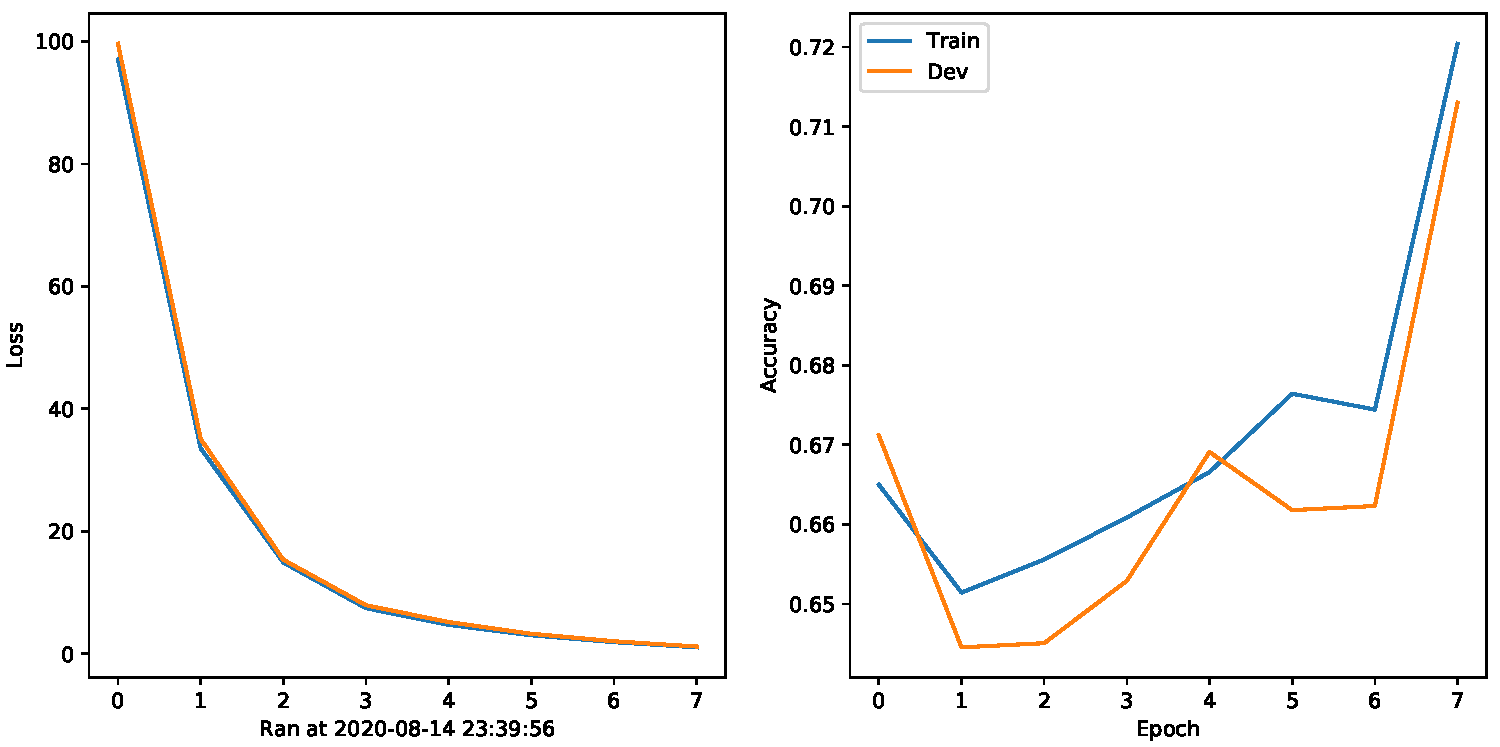
\includegraphics[scale=0.6]{./code/learning-curves.pdf} \\
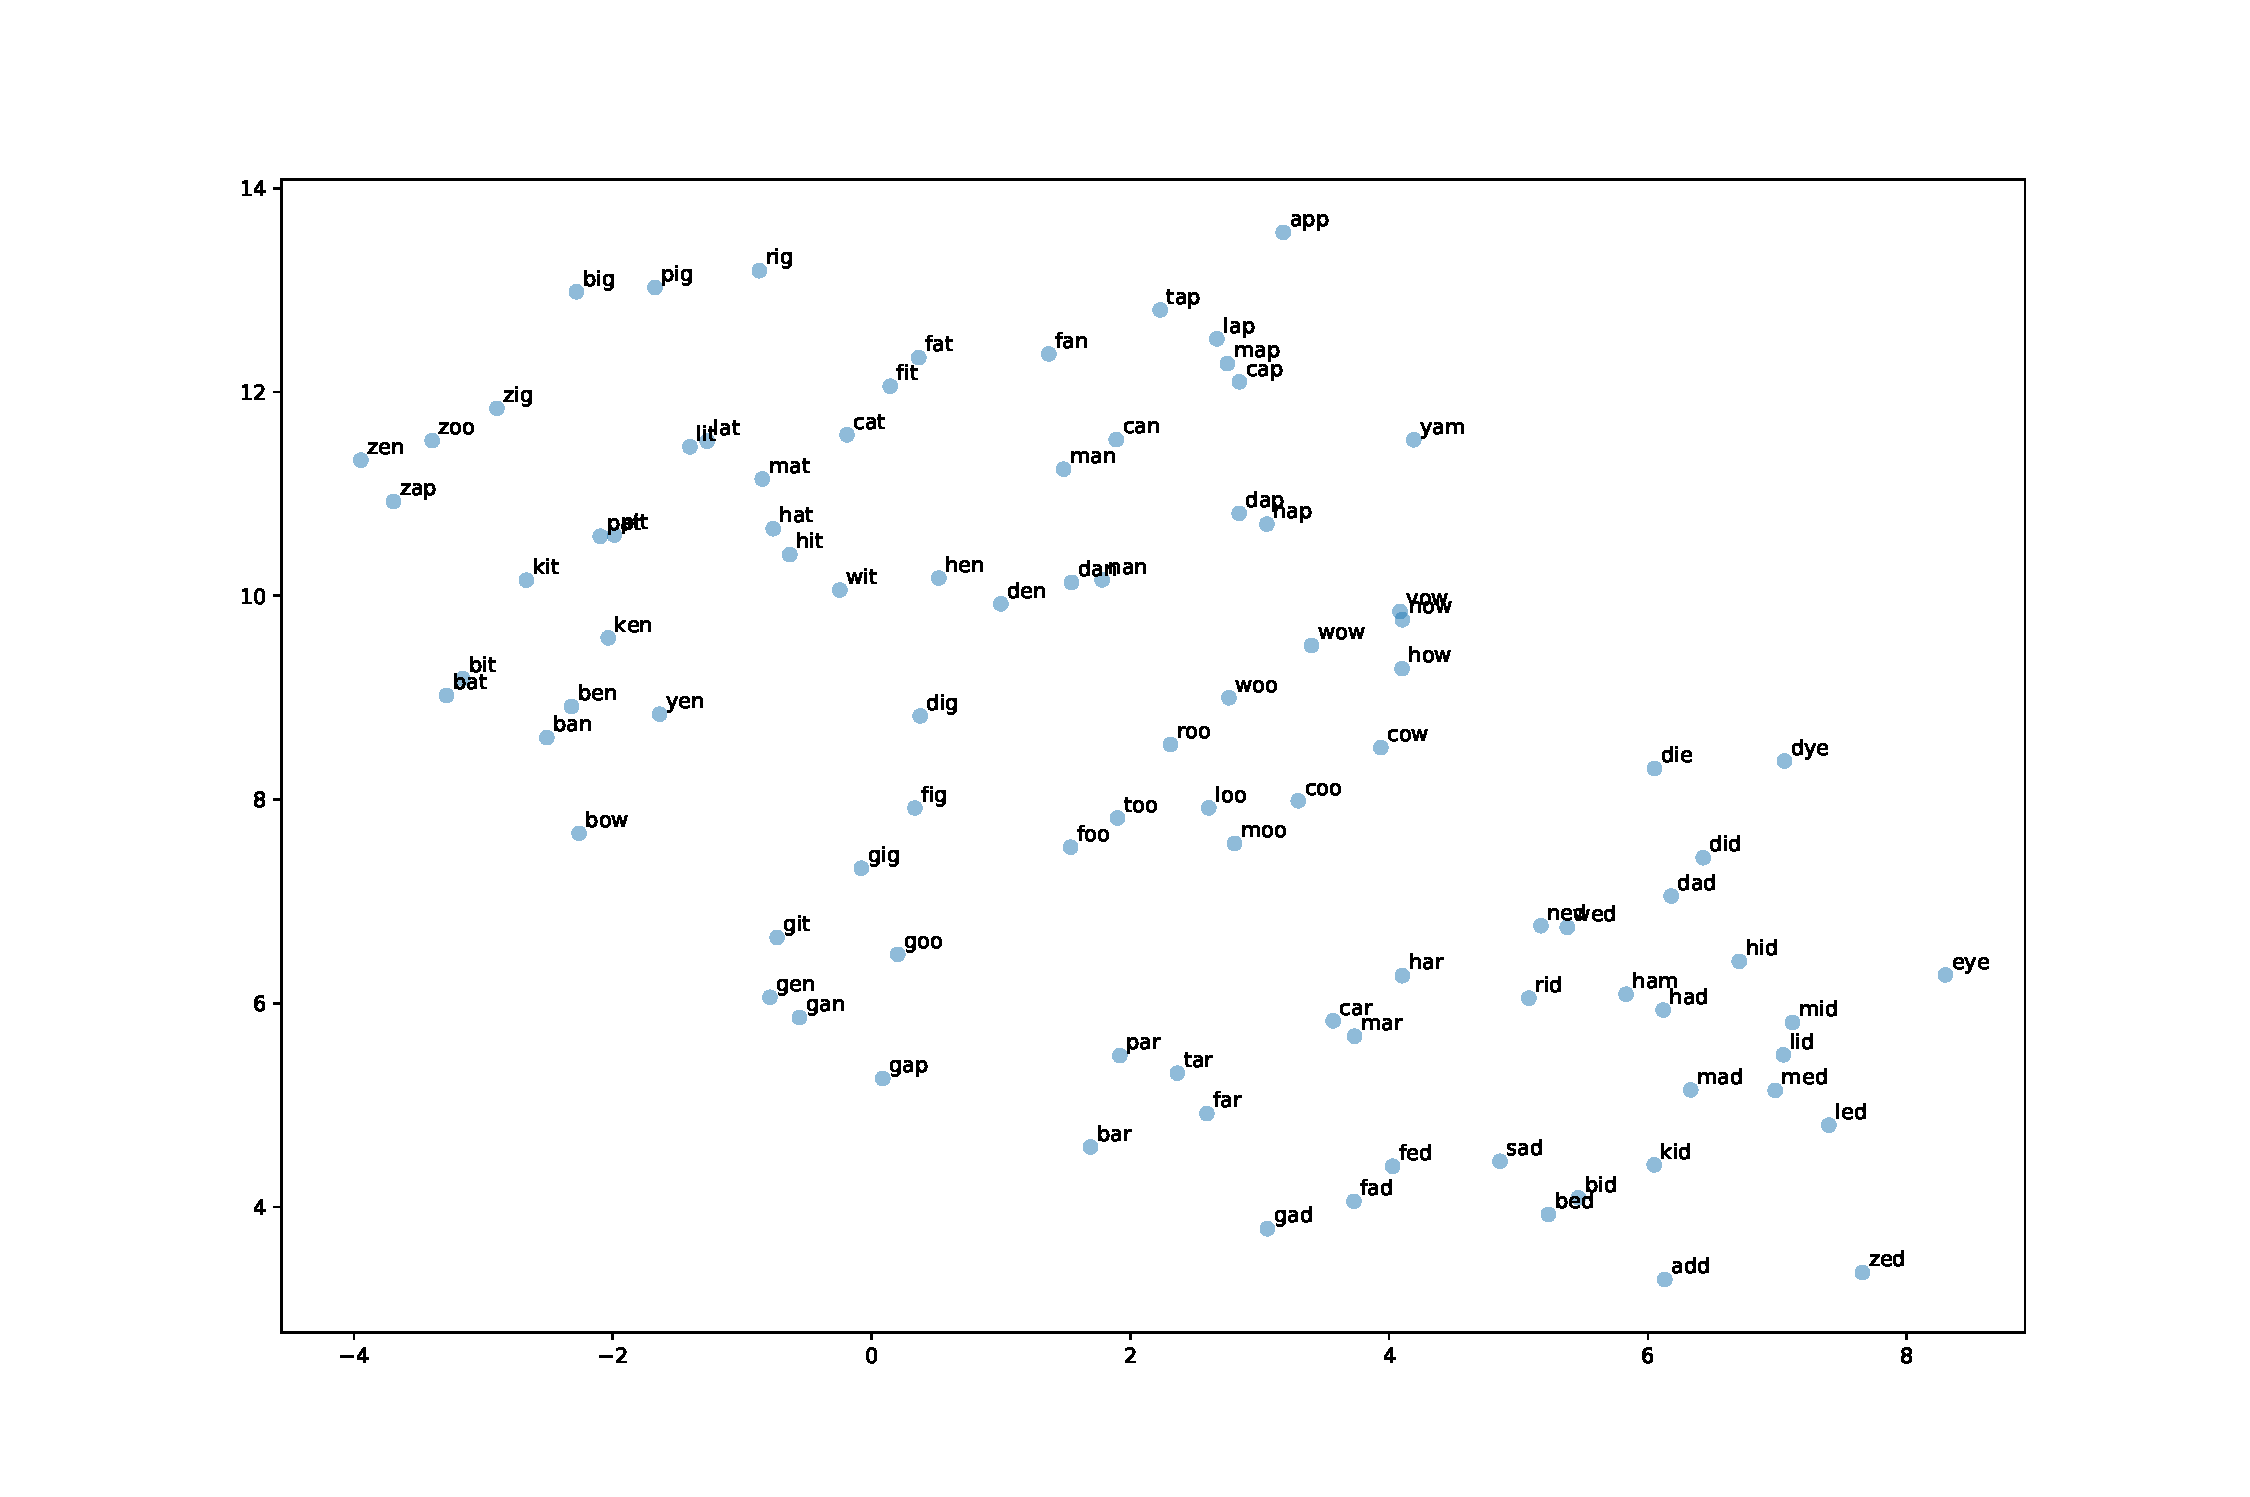
\includegraphics[scale=0.5]{./code/embeddings.pdf} \\

Phonetic Analogies:\\
"cap" is to "coo" as "zap" is to "zoo"\\
"how" is to "wow" as "hit" is to "wit"\\
"yam" is to "ham" as "yen" is to "hen"\\

}

\end{document}
